
%(BEGIN_QUESTION)
% Copyright 2007, Tony R. Kuphaldt, released under the Creative Commons Attribution License (v 1.0)
% This means you may do almost anything with this work of mine, so long as you give me proper credit

Bob Metcalfe's original Ethernet communication standard was based on ``thick'' coaxial cable.  Connections to this cable were made using coaxial ``Tee'' fittings.  

$$\includegraphics[width=15.5cm]{i02202x01.eps}$$

This approach was eventually discarded in favor of twisted-pair cabling without any mid-point taps.  With twisted-pair wiring, the end of a cable always plugged in to a piece of equipment, either DTE or DCE:

$$\includegraphics[width=15.5cm]{i02202x02.eps}$$

Explain what the purpose of the {\it hub} is, and how it is more than just a connection point like a tee fitting in the old coaxial-based cable standard. 

Note how the new hub-based approach does not require any termination resistors, even though the twisted-pair cables may be quite long (up to 100 meters).  Explain how it is possible to go without termination resistors given such long cable lengths and high data rates (100 Mbps or more!), where they were absolutely required at the ends of the old coaxial cables.

\underbar{file i02202}
%(END_QUESTION)





%(BEGIN_ANSWER)

An Ethernet {\it hub} is an active piece of communications equipment: an actual DCE, and not just a passive connector.  Inside, it contains transceiver circuits to amplify received signals and re-transmit them to the other ``ports'' on the hub.  

Termination resistors are not required with twisted-pair Ethernet networks because all Ethernet devices (DTE and DCE) are engineered with the proper termination impedance built in to the transceivers.

%(END_ANSWER)





%(BEGIN_NOTES)

This is a good example of an amplifier having a specific input and output impedance: here, the transceivers in a twisted-pair Ethernet system are designed to have the same input and output impedance as the cable needs for termination.

A definite problem with the old coax-based Ethernet is that the signal strength waned with each tap.  A long length of coax cable with lots of taps tended to degrade the strength of a signal, necessitating ``repeaters'' at occasional intervals to boost the signal.  A hub is basically a repeater, and by guaranteeing no taps in a twisted-pair network, one can guarantee good signal strength throughout the network.

%INDEX% Networking, Ethernet: hubs
%INDEX% Networking, Ethernet: twisted-pair cabling

%(END_NOTES)


